\subsection{Egérkurzor alakja}

%_
\begin{frame}
  \begin{columns}[c]
    \column{0.8\textwidth}
      \begin{itemize}
        \item Rengeteg előre beépített egérkurzor közül lehet választani a \texttt{cursor} tulajdonság értékének állításával.
        \item Saját kurzort is lehet betölteni az \texttt{url()} függvénnyel, de célszerű utána vesszővel elválasztva egy beépített kurzort is megnevezni, betöltési hiba esetére.
        \item Kurzor akár \hiv{\href{https://www.cursor.cc/}{online}} is szerkeszthető.
      \end{itemize}
    \column{0.15\textwidth}
      \begin{exampleblock}{\textattachfile{kurzor.html}{kurzor.html}, \textattachfile{cursor.cur}{cursor.cur}}
        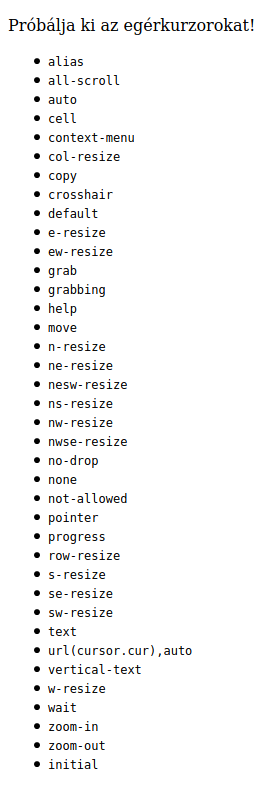
\includegraphics[width=.8\textwidth]{kurzor.png}
      \end{exampleblock}
  \end{columns}
\end{frame}
